In the last chapter I have introduced the framework of network science used to study brain networks.
I discussed the modular organization of brain networks and the graph theoretical approaches that enabled its study.
I have also shown that graph partitioning methods based on the maximization of global fitness functions, like Newman's Modularity, suffer from a fundamental resolution limit as they fail to detect modules that are smaller than a scale determined by the size of the entire graph.
Furthermore, I explored the effects of this limitation on the study of brain connectivity networks, demonstrating that the resolution limit prevents detection of important details of the brain modular structure, thus hampering the ability to appreciate differences between networks and to assess the topological roles of nodes.

In this chapter I'll show that Surprise, a recently proposed fitness function based on probability theory, does not suffer from these limitations.
I'll introduce Surprise from its theoretical foundations and discuss its properties in details.
Moreover, I'll describe an algorithm for Surprise optimization in binary graphs with an assessment of its performance on benchmark networks.
Surprise maximization in brain co-activation and functional connectivity resting state networks reveals the presence of a rich structure of heterogeneously distributed modules, and differences in networks' partitions that are undetectable by resolution-limited methods.
Moreover, Surprise leads to a more accurate identification of the network's connector hubs, the elements that integrate the brain modules into a cohesive structure.

%%%%%%%%%%%%%%%%%%%%%%%%%%%%%%%%%%%%%%%%%%%%%%%%%%%%%%%%%%%%%%%%%%%%%%%%%%%%%%%%%%%%%%%%%
%%%%%%%%%%%%%% PROBABILISTIC APPROACH TO CLUSTERING IN BINARY NETWORKS %%%%%%%%%%%%%%%%%%
%%%%%%%%%%%%%%%%%%%%%%%%%%%%%%%%%%%%%%%%%%%%%%%%%%%%%%%%%%%%%%%%%%%%%%%%%%%%%%%%%%%%%%%%%
\section{Probabilistic approach to clustering in binary networks}\label{sec:probability_clustering}
The spin-glass based additive quality functions described in the previous chapter, including Newman's Modularity, measure the deviation between the fraction of edges falling within modules and the null model. In any case though, they assess the statistical significance of this deviation.
In other terms, no spin-glass based quality function is telling us the level of statistical confidence at which one should discard the null hypothesis that the observed fraction of edges inside a community is the same as the one expected from a given null model.

To address this question, one should instead compute probabilities, as they are the natural way to measure statistical significance.
Specifically, given a node induced subgraph (a community), one is interested in computing the probability to find another subgraph having more internal edges than the observed one: the lesser the value, the more significant is the community in exam.

More precisely, the problem can be expressed as in the following: given a subgraph, what is the probability of observing another subgraph with a larger number of internal edges drawn from a random graph with a given density?
This question can be answered by the urn model in classical probability theory. The reason is clear if one imagines that each pair of nodes is a marble, which is one color if the nodes are connected by a link and the other color if they are not.
A number of marbles is drawn from an urn without replacement and the probability of observing a given number of marbles of one specific color is calculated by means of the hypergeometric law.
When applied to clustering, the problem corresponds to the calculation of the probability to observe a fixed number of internal edges in a randomly drawn set of nodes defining a community.
For example, suppose that one draws a subgraph with $n_c$ nodes, $p_c$ pairs of nodes and $m_c$ edges from a graph with $n$ nodes, $p$ pairs of nodes and $m$ edges (see Section for the notation~\ref{sec:clustering}).
As indicated by the urn model, the probability to observe exactly $m_c$ internal edges is given by:
\begin{equation}\label{eq:subgraph_probability}
\Pr[i=m_c] = \frac{\binom{m}{i}\binom{p-m}{p_c-i} }{\binom{p}{p_c}} = \frac{\binom{p_c}{i} \binom{p-p_c}{m-i}}{\binom{p}{m}}
\end{equation}
where the last equality is because of the Vandermonde identity~\cite{feller1968}.
The probability in Eq.~\ref{eq:subgraph_probability} is simply understood in terms of urn model as there are $\binom{p_c}{i}$ ways of choosing exactly $i$ black marbles from a population of $p_c$ black marbles, $\binom{p-p_c}{m-i}$ ways of choosing $(m-i)$ white marbles from a population of $(p-p_c)$ white marbles and a total possible number of combinations of $m$ marbles taken from a population of $p$ of them. Figure~\ref{fig:subgraphconditionalprobability} shows an example where the probability of randomly picking the subgraph $\mathcal{G}$ from the graph $G$ is computed by means of the urn model.
\begin{figure}[htb]
\centering
\begin{tikzpicture}
%\draw[help lines,step=1] (-4,-4) grid (8,4);
\draw [rectangle, black, draw, rounded corners=2ex,line width=0.25ex] (1.6,-0.5) rectangle (3.4,1.5);

\draw (1,0) -- (3,0);
\draw (2,1) -- (3,1) -- (2,0) -- (3,0) -- cycle;
\node [fill=gray!30, radius=1ex, draw, circle, inner sep=2pt] at (2,1) {$e$};
\node [fill=gray!30, radius=1ex, draw, circle, inner sep=2pt] at (3,1) {$f$};
\node [fill=gray!30, radius=1ex, draw, circle, inner sep=2pt] at (2,0) {$g$};
\node [fill=gray!30, radius=1ex, draw, circle, inner sep=2pt] at (2,0) {$g$};
\node [fill=gray!30, radius=1ex, draw, circle, inner sep=2pt] at (3,0) {$h$};
\draw (0,1) -- (1,1);
\draw (1,1) -- (1,0);
\draw (1,0) -- (1,1);
\draw (1,1) -- (0,0);
\node [fill=gray!30, radius=1ex, draw, circle, inner sep=2pt] at (0,1) {$a$};
\node [fill=gray!30, radius=1ex, draw, circle, inner sep=2pt] at (1,1) {$b$};
\node [fill=gray!30, radius=1ex, draw, circle, inner sep=2pt] at (0,0) {$c$};
\node [fill=gray!30, radius=1ex, draw, circle, inner sep=2pt] at (1,0) {$d$};
\node at (2.5,1.75) {$\mathcal{G}$};
\node at (0.5,1.75) {{\color{red}$G-\mathcal{G}$}};
\draw [rectangle, red, draw, rounded corners=2ex,line width=0.25ex] (-0.4,-0.5) rectangle (1.4,1.5);
\node [] at (5.5,1) {$\Pr(\mathcal{G}) = \dfrac{\binom{6}{4} \binom{28-4}{10-6}}{\binom{28}{10}}$};
\node [] at (6.0,0) {$\approx 0.0121$};

\node [] at (9.5,1) {$m_c=4,p_c=6,n_c=4$};
\node [] at (9.5,0) {$p=28,m=10,n=8$};
\end{tikzpicture}
\caption{Probability for the subgraph $\mathcal{G}=(\mathcal{V},\mathcal{E})$ where $\mathcal{V}=\{e,f,g,h\}$ and $\mathcal{E}=\{(e,f),(f,g),(g,h),(e,h)\}$ to be randomly drawn from the graph $G$.}
\label{fig:subgraphconditionalprobability}
\end{figure}
As the probability of observing $i$ or more internal edges, is given by the sum of the probabilities of observing exactly $i$,$i+1$,$i+2$ etc. internal edges, summing on $i$ yields the probability of getting \emph{at least} $m_c$ white marbles:
\begin{equation}\label{eq:subgraph_probability_marginalized}
\Pr[ m_c \geq i ] = \sum\limits_{i=m_c}^{m} \frac{\binom{p_c}{i} \binom{p-p_c}{m-i}}{\binom{p}{m}}
\end{equation}

In this last equation we are considering the probability of randomly drawing a subgraph with $m_c$ or more internal edges over the set of all random subgraphs with $n$ nodes and exactly $m$ edges as in the $G_{nm}$ model described in section~\ref{sec:models_random_graph}. Indeed, the denominator $\binom{p}{m}$ in Equation~\ref{eq:subgraph_probability_marginalized} represent the possible number of graphs with $p$ pairs of nodes and $m$ edges. 

%%%%%%%%%%%%%%%%%%%%%%%%%%%%%%%%%%%%%%%%%%
%%%%%%%%%%%%%% SURPRISE %%%%%%%%%%%%%%%%%%
%%%%%%%%%%%%%%%%%%%%%%%%%%%%%%%%%%%%%%%%%%
\section{Surprise}
The intuition captured by Eq.~\ref{eq:subgraph_probability_marginalized} is very close to a quality function dubbed \emph{Surprise}, firstly introduced in a seminal paper by Aldecoa and Marin~\cite{aldecoa2011}.
Yet, to the best of my knowledge, this clearer theoretical motivation did not appear in any other works.
If one considers as the random subgraph that is drawn from the $G_{n,m}$ set, a subgraph with at least $m_\zeta=\sum_c m_c$ internal edges and $p_\zeta=\sum_c p_c$ pairs of edges, then this subgraph represents a whole clustering.
In this case, the definition given in Eq.~\ref{eq:subgraph_probability_marginalized} and the definition given in~\cite{aldecoa2011} are perfectly corresponding.
Indeed, for a partition $\zeta$, the probability that a subgraph $\mathcal{G}$ randomly drawn from the set $G_{nm}$ has at least $m_\zeta$ intracluster edges and $p_\zeta$ intracluster pairs is modeled after the inverse cumulative hypergeometric distribution, exactly as in~\ref{eq:subgraph_probability_marginalized}.
Here and in the rest of the work, the quality function \emph{Surprise} is therefore expressed by the following definition:
\begin{equation}\label{eq:surprise}
S(\zeta) := \sum_{i = m_\zeta}^m \dfrac{\binom{p_\zeta}{i} \binom{p-p_\zeta}{m-i} }{\binom{p}{m}}
\end{equation}

Surprise computes the probability to (surprisingly) observe at least as many internal edges as within the proposed partition in a uniform random graph.
As mentioned, model in Eq.~\ref{eq:surprise} corresponds to an urn model without reinsertion, where $S$ is the probability of extracting at least $m_\zeta$ white balls out of $m$ trials from an urn containing $p_\zeta$ white balls and $p-p_\zeta$ black balls.
Intuitively, the lower $S(\zeta)$, the better the clustering. Optimal partitions with respect to $S$ are those with the highest number of intracluster edges and the smallest number of intracluster pairs. 

Differently from Modularity, $S(\zeta)=1$ both for the partition where every node is in a separated community ($|\zeta|=n$,$p_\zeta=0$,$m_\zeta=0$) and for the partition that entails all nodes into a single group ($|\zeta|=1$,$p_\zeta=p$,$m_\zeta=m$) as is evident from its formulation in terms of urn model.
Indeed, as Newman's Modularity is zero when $|\zeta|=1$, and different from zero in the case $|\zeta|=n$.
In terms of Surprise both the extreme partitions are instead equally uninformative and assigned to $S=1$ (or equivalently $\hat{S}=0$).
Indeed, for the case of a single community comprising all nodes, the probability of observing a number of intracluster edges greater or equal than the number of edges is one. On the other hand, if the partitioning has zero intracluster edges as for the case of $n$ separate communities, the probability to observe more than zero intracluster edges is still one.

It should be noted that, due to numerical precision problems in the evaluation of large binomial coefficients, $\hat{S}(\zeta) := -\log_{10}S(\zeta)$ is often taken as measure of quality of the partition, which is totally equivalent with respect to optimum solutions, where higher values correspond to better clustering.
Different authors~\cite{arnauVMarsS2005,fleck2014} refer to $S$ as Surprise, whereas others~\cite{aldecoa2011,aldecoa2013} use $\hat{S}$. Hereafter I stick to the notation of~\cite{fleck2014} where Surprise is indicated as $S$ defined in Eq.~\ref{eq:surprise} and indicate $\hat{S}$ where needed.

%%%%%%%%%%%%%%%%%%%%%%%%%%%%%%%%%%%%%%%%%%%%%%%%%%%%%%%%%%%%%%
%%%%%%%%%%%%% STATISTICAL TEST INTERPRETATION %%%%%%%%%%%%%%%%
%%%%%%%%%%%%%%%%%%%%%%%%%%%%%%%%%%%%%%%%%%%%%%%%%%%%%%%%%%%%%%
\subsection{Statistical test interpretation}
\label{sec:surprisefishertest}
Surprise considers the problem of community detection as the one of making the intracluster density as further as possible from the global density in statistical terms.
In this sense, it's worth noting that $S$ is \emph{p}-value of a one-tailed Fisher exact-test where one is asking how confidently should reject the null hypothesis $H_0$ that the intracluster density is the same as the graph density.
It turns indeed out that this problem has an equivalent description in statistics, where one seeks to maximize the \emph{odds-ratio} of the $2 \times 2$ contingency table defined in Table~\ref{tab:contingency_table}.

The Fisher exact test implemented by Surprise is, as its name states, exact as long as the contingency table keeps the row and column totals fixed, and it can therefore be used regardless of the sample characteristics.
A simpler $\chi^2$ statistic can be used when the elements of the contingency table are large enough, although only an approximation of the \emph{p}-value can be obtained.
In this case it's possible to tackle the problem of computation of $S$ by means of odds-ratio.
Precisely, the \emph{normalized log odds-ratio} is computed as: 
\begin{equation}
\log(\textrm{OR}) = \log\left( \frac{m_\zeta(p-m-p_\zeta+m_\zeta)}{(m-m_\zeta)(p_\zeta-m_\zeta)} \right ),
\end{equation}
and in the asymptotic case, Surprise is equal to the probability:
\begin{equation}\label{eq:prob_or_se}
\Pr\left(z < -\frac{|\log\textrm{OR})|}{SE} \right)
\end{equation}
where $z$ is a random variable with standard normal distribution $z \approx \mathcal{N}(0,1)$ and $SE$ is the standard error of the odds-ratio, approximately computed as 
\begin{equation}
SE=\sqrt{\frac{1}{m_\zeta} + \frac{1}{(p_\zeta-m_\zeta)} + \frac{1}{(m-m_\zeta)} + \frac{1}{(p - m - p_\zeta + m_\zeta)}}.
\end{equation}
Although not interesting in the case of binary graphs, Equation~\ref{eq:prob_or_se} is telling us that in developing a version of Surprise that will keep into account weighted graphs, we should in some way rely on its asymptotic distribution.

\begin{table}[htb!]
\centering
\begin{tabular}{|c|c|c|c|}
\hline
 & Drawn & Not drawn & \textbf{Total}\\
\hline
Intracluster & $m_\zeta$ & $p_\zeta-m_\zeta$ & $p_\zeta$\\
\hline
Intercluster & $m-m_\zeta$ & $p-m-p_\zeta+m_\zeta$ & $p-p_\zeta$ \\
\hline
\textbf{Total} & $m$ & $p-m$ & $p$ \\
\hline
\end{tabular}
\caption{Contingency table for the urn model.}
\label{tab:contingency_table}
\end{table}

%%%%%%%%%%%%%%%%%%%%%%%%%%%%%%%%%%%%%%%%%%%%%%%%%%%%%%%%%%%%%%%%%%%%%%%%%%%%%%%%%%%%
%%%%%%%%%%%%%%%%%%%%%%%%%%%% GENERAL PROPERTIES OF SURPRISE %%%%%%%%%%%%%%%%%%%%%%%%
%%%%%%%%%%%%%%%%%%%%%%%%%%%%%%%%%%%%%%%%%%%%%%%%%%%%%%%%%%%%%%%%%%%%%%%%%%%%%%%%%%%%
\subsection{General properties of Surprise}
As noted by~\cite{fleck2014}, for a given graph, $m$ and $p$ are fixed so $S(\zeta)$ is depending only on the number of intracluster edges $m_\zeta$ and intracluster pairs $p_\zeta$, namely $S:=S(m_\zeta,p_\zeta)$.
In establishing the domain of validity of $(m,p,m_\zeta,p_\zeta)$ the urn model is of help. A valid clustering $\zeta$ of mutually disjoint communities automatically satisfies intuitive but important requirements:
\begin{obs}
It's impossible to draw more white balls than the white balls contained in the urn, therefore $p_\zeta \geq m_\zeta$.
\end{obs}
\begin{obs}
It's impossible to have more white balls than total number of drawn balls, therefore $m\geq m_\zeta$.
\end{obs}
\begin{obs}
It's impossible to draw more black balls than the black balls contained in the urn, therefore $p-p_\zeta \geq m-m_\zeta$.
\end{obs}
All valid clusterings are enclosed inside the domain $\mathcal{L}$ defined as from these last three observation:
\begin{equation}
\mathcal{L} := \{ ( m_\zeta,p_\zeta) \; | m_\zeta > 0 \land p_\zeta \geq m_\zeta \land m \geq m_\zeta \land p-m > p_\zeta - m_\zeta \}
\end{equation}
The urn models gives other three important properties, indicating that Surprise is a convex function inside the domain of validity of its variables. Specifically as shown in~\cite{fleck2014} three inequalities apply for Surprise and for the urn model in general.
\begin{props}\label{prop:prop1}
\label{list:surprise_properties} It's less probable to draw at least $m_\zeta+1$ than $m_\zeta$ white balls if the urn contains the same number of $p_\zeta$ white balls, therefore $S(m_\zeta+1,p_\zeta) < S(m_\zeta,p_\zeta)$.
\end{props}
\begin{props}\label{prop:prop2}
It's less probable to draw at least $m_\zeta$ white balls if the urn has one white balls less, therefore $S(m_\zeta,p_\zeta-1) < S(m_\zeta,p_\zeta)$.
\end{props}
\begin{props}\label{prop:prop3}
It's less probable to draw at least $m_\zeta+1$ white balls if the urn has $p_\zeta+1$ white balls, than drawing at least $m_\zeta$ white balls if the urn has $p_\zeta$ white balls, therefore $S(m_\zeta+1,p_\zeta+1) < S(m_\zeta,p_\zeta)$.
\end{props}
The scheme in Figure~\ref{fig:surprisebehaviour} shows the order relation between the elements of the three aforementioned inequalities.
\begin{figure}[htb]
\centering
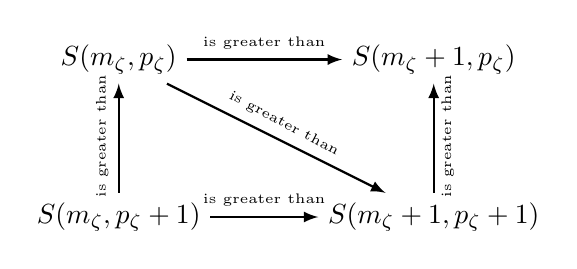
\begin{tikzpicture}
  \node[] (S00) at (0,0) {$S(m_\zeta,p_\zeta)$};
  \node[] (S10) at (4,0) {$S(m_\zeta+1,p_\zeta)$};
  \node[] (S01) at (0,-2) {$S(m_\zeta,p_\zeta+1)$};
  \node[] (S11) at (4,-2) {$S(m_\zeta+1,p_\zeta+1)$};
  \draw[->,thick,>=latex] (S00) -- node[anchor=south] {\tiny{is greater than}} (S10);
  \draw[->,thick,>=latex] (S01) -- node[anchor=south] {\tiny{is greater than}} (S11);
  \draw[->,thick,>=latex] (S11) -- node[anchor=west,xshift=5,yshift=-25,rotate=90] {\tiny{is greater than}} (S10);
  \draw[->, thick,>=latex] (S00) -- node[anchor=south,rotate=-28] {\tiny{is greater than}} (S11);
  \draw[->,thick,>=latex] (S01) -- node[anchor=west,xshift=-6,yshift=-25,rotate=90] {\tiny{is greater than}} (S00);
\end{tikzpicture}
\caption{Behaviour of the landscape of Surprise $S$.}
\label{fig:surprisebehaviour}
\end{figure}

A fourth inequality $S(m_\zeta,p_\zeta+1)>S(m_\zeta+1,p_\zeta)$ is implicit by looking at the behaviour of $S(\zeta)$ for a given graph. 
The scheme in Figure~\ref{fig:surprisebehaviour} allows to rank the values of Surprise in relation to changes in $m_\zeta$ and $p_\zeta$.
It's to easy verify that $S$ satisfies the following strict order relation:
\begin{equation}\label{eq:surpriseorderrelation}
S(m_\zeta+1,p_\zeta)<S(m_\zeta+1,p_\zeta+1)<S(m_\zeta,p_\zeta)<S(m_\zeta,p_\zeta+1).
\end{equation}
This property led me to the observation that Surprise $S$ is a monotonically decreasing function (increasing $\hat{S}$) of $m_\zeta$ and monotonically increasing function (decreasing $\hat{S}$) of $p_\zeta$ in the convex interval $\mathcal{L}$.
Moreover, from Figure~\ref{fig:surprisebehaviour} follows that optimal solutions with respect to $S$ are Pareto-optimal with respect to maximizing $m_\zeta$ and minimizing $p_\zeta$.
In other words, a partition that is optimum with respect to Surprise is such that no further increment in $m_\zeta$ leads to a decrement in $p_\zeta$ that has higher $\hat{S}$.
The Pareto optimality of optimum Surprise partitions, implies that a perturbation of $\delta m_\zeta, \delta p_\zeta$ leads to a change in Surprise such that it monotonically decreases if and only if $\delta m_\zeta > \delta p_\zeta$, precisely:
\begin{equation}\label{eq:resolution_limit_condition}
S(m_\zeta + \delta_{m_\zeta}, p_\zeta + \delta_{p_\zeta}) < S(m_\zeta,p_\zeta) \iff \delta_{m_\zeta} \geq \delta_{p_\zeta}.
\end{equation}

%% \begin{figure}[htb!]
%% \centering
%% \begin{tikzpicture}[scale=0.8, every node/.style={scale=0.8}]
%% \def \S {1};
%% \def \W {11};
%% \def \H {7};
%% \node[anchor=south west, inner sep=0mm] at (0,0) { \includegraphics[width=\W cm]{images/plot_surprise_pareto.pdf}};
%% \node[anchor=south] at (\W /2,\H +0.25) {$\hat{S}=-\log_{10}(S(m_\zeta,p_\zeta$, $m=10$,$p=15$))};
%% %\draw[help lines,xstep=1.0,ystep=1.0] (0,0) grid (\W,\H);
%% \foreach \x in {1,...,\W } {\node [anchor=north] at (\x-0.5,0) {$\x$}; }
%% \node[anchor=north] at (\W/2,-0.5){$p_\zeta$};
%% \foreach \y in {1,...,\H} {\node [anchor=east] at (0 ,\y-0.5) {$\y$}; }
%% \node[anchor=east] at (-0.5,\H/2){$m_\zeta$};
%% %\node[rectangle,fill=black!10,draw=black,rounded corners=0.1cm] at (\W+1.5,\H-0.5) {$m_{\zeta},p_\zeta \not \subset \mathcal{L}$};
%% \end{tikzpicture}
%% \caption{Pareto optimality of Surprise (here $\hat{S}$ is represented) on a trivial graph with $n=6$ nodes and $m=7$ edges. No increment in $m_\zeta$ leads to a decrement in $p_\zeta$ that has higher $\hat{S}$. Here Surprise is optimal for $m_\zeta=6,p_\zeta=6$.}
%% \label{fig:pareto_optimality_surprise}
%% \end{figure}
%% \todo[inline]{CONTROLLARE FIGURA PROBABILMENTE SBAGLIATA PERCHE MZETA>M!!!}

The result in Eq.\ref{eq:resolution_limit_condition} is of great help in designing optimization algorithms as every move that increase the intracluster edges more than intracluster pairs is good, while moves that increase intracluster pairs more than intracluster edges must be ignored, therefore sparing time for the computation of Surprise. Additionally, Eq.~\ref{eq:resolution_limit_condition} is useful when analyzing the onset of the resolution limit for different models.
In the next sections I will show to what extent Surprise is affected by the resolution limit for Surprise, to show with convincing theoretical arguments that $S$ is nearly resolution-limit-free in Traag's sense~\cite{traag2015}.

%%%%%%%%%%%%%%%%%%%%%%%%%%%%%%%%%%%%%%%%%%%%%%%%%%%%%%%%%%%%%%
%%%%%%%%%%%% RESOLUTION LIMIT AND SURPRISE %%%%%%%%%%%%%%%%%%%
%%%%%%%%%%%%%%%%%%%%%%%%%%%%%%%%%%%%%%%%%%%%%%%%%%%%%%%%%%%%%%
\section{Resolution limit and Surprise}
Unfortunately, the resolution limit is an intrinsic feature of many quality functions, and there appears to be a ``narrow scope to resolution-limit-free methods''~\cite{traag2015}.
Surprise has been shown to outperform other network partitioning methods in the detection of small features within large graphs, but the extent to which it suffered from the resolution limit was unknown~\cite{aldecoa2011,aldecoa2013}, until our work~\cite{nicolini2016}.

Aldecoa~\cite{aldecoa2011}, pointed out that while Modularity-based methods define a community as a region with an unexpectedly high density of links with respect to the global characteristics of the network, Surprise weights the number of actual intracluster edges against the maximum number of links given the nodes in the clusters.
Hence, Surprise is able to discriminate local subnetworks whose internal density is close to that of a clique independently of their size.

In order to assess the extent to which Surprise is affected by the resolution limit, I directly compared Newman's Modularity and Surprise in the example of Fortunato and Barthelemy illustrated in the previous chapter in Figure~\ref{fig:figure_1_barthelemy}. Already for $m_{12} = 1$, i.e. when the two cliques $G_1$ and $G_2$ were connected by only one edge, $Q^N$ showed sign inversion for $m_0 \approx 200$, meaning that it was beneficial for Modularity to merge two cliques.
In this same example, Surprise never merges cliques, as shown in Figure~\ref{fig:barthelemy_surprise}.

\begin{figure}[htb!]
\centering
\includegraphics[width=1.0\textwidth]{images/barthelemy_surprise.pdf}
\caption{Difference in $\hat{S}$ between the partition where the two cliques are separated (red) and the partition where the two cliques are merged (blue), as in the benchmark network of Fortunato and Barthelemy. As the quantity $\Delta \hat{S}$ is always positive, Surprise is never going to merge cliques, independently from other global parameters. Adapted from Nicolini and Bifone~\cite{nicolini2016}.}
\label{fig:barthelemy_surprise}
\end{figure}

Figure~\ref{fig:barthelemy_surprise} shows that Surprise does not suffer from the resolution limit at least in this specific case.
Indeed, $\Delta \hat{S}$ is always positive and grows monotonically with increasing $m_0$. 
Hence, the two cliques $G_1$ and $G_2$ are always resolved by Surprise as separate communities independently of the network size, and also in the presence of some ``fuzziness'', i.e. when $m_{12}>1$ and the two cliques are connected by more than one edge.
In order to assess whether this behavior reflects a general property of Surprise, or is incidental to this particular example, I have also studied a generalization of Fortunato and Barthelemy's model.

A consequence of the definition of a resolution limit free quality function in Traag's sense, is that such method will never depend on the size of the network to merge cliques in a graph comprising $r$ cliques of $n_r$ nodes connected in a ring structure as in Figure~\ref{fig:traag_ring_of_cliques} (often called the ``ring of cliques'' model).
This observation prompted me to explore the behavior of $\hat{S}$ in the ring of cliques model graph, as an extension of Fortunato and Barthelemy's model.
Interestingly, given its two-variables formulation, Surprise optimization can be seen as a multiobjective optimization problem where one seeks to minimize the intracluster pairs while maximizing the number of intracluster edges.
With increasing graph size, the computational problem of calculating $\hat{S}$ for every possible partition becomes rapidly intractable (maximization of $S$ is NP hard)~\cite{fleck2014}.
However, as explained before and pointed out by Fleck et al.~\cite{fleck2014}, the Surprise optimal clustering must be Pareto optimal with respect to minimizing $p_\zeta$ and maximizing $m_\zeta$, i.e. any further improvement in one of the two variables must occur at the expense of the other.

In this sense, the problem of Surprise optimization is shown to be equivalent to a linear program~\cite{fleck2014}, where one seeks to minimize $p_\zeta$ while keeping $m_\zeta$ equal to a constant $h$ from $1$ to $m$, choosing then among the resulting $m$ clusterings, the one that maximizes $\hat{S}$.
Hence, to delineate the Pareto frontier in the $(m_\zeta,p_\zeta)$ space, we need to solve $m$ integer linear programs (ILP) in the form:
\begin{align}\label{eq:surprise_ilp}
\textrm{minimize} \sum_{\{i,j\} \in \binom{V}{2}} \mathcal{X}_{ij} \nonumber \\
\textrm{s.t.} \quad \mathcal{X}_{ij} \in \{0,1 \} \nonumber \\
\quad \mathcal{X}_{ik} + \mathcal{X}_{ki} - \mathcal{X}_{ij} \leq 1 \nonumber \\
\sum_{\{i,j\} \in E} \mathcal{X}_{ij}=h \nonumber
\end{align}
where $\mathcal{X}_{ij}$, equivalent to $\delta(\sigma_i, \sigma_j)$, are a set of $\binom{n}{2}$ binary variables corresponding to vertex pairs, with the interpretation that $\mathcal{X}_{ij}=1$ if vertex $i$ and vertex $j$ are in the same community. The alternative objective function $\sum_{ij}\mathcal{X}_{ij}$ measures the number of intracluster pairs $p_\zeta$, while the number of intracluster edges $m_\zeta=\sum_{ij \in E} \mathcal{X}_{ij}$ was set equal to a fixed $h \in [0,m]$. The remaining constraints are necessary in order to ensure transitivity, i.e. if nodes $i$ and $j$ are in the same community, nodes $i$ and $k$ are in the same community, then nodes $j$ and $k$ share the same community too. 
Figure~\ref{fig:ring_cliques_pareto} shows the Pareto frontier for a ring of cliques where I independently varied the number of cliques $r$ and the number of nodes $n$ in every clique\footnote{Linear programs were solved using the Python interfaces of Gurobi 5.7.3 on Linux (Gurobi Optimizer Version 5.7, Gurobi Optimization, Inc., Houston, Texas, United States).}.
As $\hat{S}$ reaches its minimum (zero) both in the case where all nodes are separated communities ($p_\zeta=0$) or when a single community entails all nodes ($p_\zeta=p$), Figure~\ref{fig:ring_cliques_surprise} shows monotonically increasing Surprise along the frontier with increasing $p_\zeta$ up to the Surprise optimum, indicated by black circles in the Pareto front of Figure~\ref{fig:ring_cliques_pareto}, whereas the corresponding partition identified each clique as a separate community.
Importantly, in the range of parameters I have investigated, Surprise optimization never merged cliques in the ring of cliques, independently of the size of the graph, and behaved as a Traag's resolution-limit free method.

\begin{figure}[htb!]
\centering
\includegraphics[width=0.75\textwidth]{images/ring_cliques_pareto.pdf}
\caption{Pareto front for a ring of cliques graph. Optimal solutions with respect to Surprise are indicated as small black dots. Adapted from Nicolini and Bifone~\cite{nicolini2016}.}
\label{fig:ring_cliques_pareto}
\end{figure}
\begin{figure}[htb!]
\centering
\includegraphics[width=0.75\textwidth]{images/ring_cliques_surprise.pdf}
\caption{Surprise $\hat{S}$ for a ring of cliques graph at different levels of $p_\zeta$ for corresponding solutions at fixed $m_\zeta$. The peak of $\hat{S} $is always reached at $p_\zeta$ when the modules entail single cliques separately. Adapted from Nicolini and Bifone~\cite{nicolini2016}.}
\label{fig:ring_cliques_surprise}
\end{figure}
While it is likely that this property is quite general and can be extended to every ring of cliques, an analytical demonstration is hampered by the non-additivity of the Surprise function.
Nonetheless, the size of the graphs explored numerically is quite typical of brain-connectivity networks and I felt encouraged to apply Surprise maximization to the study of the community structure of the brain.

%%%%%%%%%%%%%%%%%%%%%%%%%%%%%%%%%%%%%%%%%%%%%%%%%%%%%%%%%%%%%%%%%%%%%%%%%%%%%%%%%%%%
%%%%%%%%%%%%%%%%%%%%%%% DEGENERACY OF SURPRISE  %%%%%%%%%%%%%%%%%%%%%%%%%%%%%%%%%%%%
%%%%%%%%%%%%%%%%%%%%%%%%%%%%%%%%%%%%%%%%%%%%%%%%%%%%%%%%%%%%%%%%%%%%%%%%%%%%%%%%%%%%
\section{Degeneracy of Surprise}\label{sec:degeneracy_surprise}
Interestingly, the maximum value of Surprise for given $(m_\zeta,p_\zeta)$ is sharply peaked and very different from other partitions, indicating that at least in this case Surprise shows no degeneracy of optimal solutions, as instead shown for Modularity in Section~\ref{sec:degeneracy}.
This observation led us to investigate to what extent Surprise is affected by the degeneracy problem.
We repeated the procedure indicated in section~\ref{sec:degeneracy}, where I embedded the complex landscape of partitions in a three dimensional space in order to show whether optimal Surprise solutions group in a large plateau of high Surprise values or not. The global optimum is a sharply distinct partition, sitting on top of the embedded manifold, as illustrated in Figure~\ref{fig:degeneracy_surprise}.
\todo{mettere conclusioni degeneracy}
\begin{figure}[ht]
\centering
\includegraphics[height=0.4\textwidth]{images/degeneracy_surprise_n_5_c_24.png}\hfill
\includegraphics[height=0.4\textwidth]{images/degeneracy_surprise_n6_c30.png}
\caption{Degeneracy of Surprise landscape in a small (left) and large (right) ring of cliques graph. No plateaus exist, indicating the uniqueness of the global maximum that emerges from the other local optima.}
\label{fig:degeneracy_surprise}
\end{figure}

%%%%%%%%%%%%%%%%%%%%%%%%%%%%%%%%%%%%%%%%%%%%%%%%%%%%%%%%%%%%
%%%%%%%%%%%% MAXIMIZATION OF SURPRISE: FAGSO %%%%%%%%%%%%%%%
%%%%%%%%%%%%%%%%%%%%%%%%%%%%%%%%%%%%%%%%%%%%%%%%%%%%%%%%%%%%
\section{Maximization of Surprise: FAGSO}\label{sec:max_surprise_fagso}

Community detection is a NP-hard problem, and heuristics have to be developed for the optimization of quality functions for relatively large networks. In their original paper, Aldecoa et al.~\cite{aldecoa2011} applied metaheuristics, involving the evaluation of Surprise for partitions resulting from seven different community detection methods, each of those maximizing different quality functions.
Here, I describe direct maximization of Surprise by exploiting FAGSO~\cite{jiang2014} (Fast AGlomerative Surprise Optimization), an agglomerative optimization algorithm that builds on a variation of the Kruskal algorithm for minimum spanning tree~\cite{leiserson2001}.
The detailed pseudocode of this algorithm is reported in Algorithm~\ref{alg:fagso} and illustrated step by step on an example network in Figure~\ref{fig:fagso_working}.

The first step of FAGSO consists in ranking the edges in the graph in decreasing order by the Jaccard index of the neighbors of their two endpoints nodes.
An union-find data structure is used to hold the community structure throughout the computation.
At the beginning, each community consists only of one vertex.
Then, starting from the edge with the highest Jaccard index at the top of the list, the endpoints are attributed to the same community by disjoint-set union if this operation leads to a strictly better Surprise and if they do not belong already in the same community.
This step is repeated for all edges and the final community structure is returned in the disjoint-set.
FAGSO finds partitions with high Surprise and it is deterministic, unless two edges with the same Jaccard index are found. In this case, ties are broken at random. 
The implementation of FAGSO in \texttt{C++}, \texttt{Python} and \texttt{GNU Octave} is freely available at \url{https://github.com/carlonicolini/fagso}.
\begin{Algorithm}[htb!]
%%%% FAGSO %%%%
\begin{small}
\begin{codebox}
\Procname{$\proc{Fagso}(G)$}
\li $S\gets 0$ \Comment \emph{Initialize Surprise to $0$}
\li $D \gets \emptyset$ \Comment \emph{Initialize disjoint set forest}
\li \For each vertex $v$ in $V[G]$
\li \Do \proc{Make-Set}(v)
\End
\li $E' \gets \proc{Sort-Jaccard}(E)$ \Comment \emph{Sort edges in decreasing order by Jaccard index}
\li \For each edge$(u,v) \in E'$, \Comment \emph{Taken in decreasing order by Jaccard index}
\li \Do \If $\proc{Find-Set}(u) \neq \proc{Find-Set}(v)$
\li \Then \If $\proc{Surprise}(G,D \cup \{ (u,v)\} ) > S$
\li $D \gets D \cup  \{(u,v)\}$
\li $\proc{Union(u,v)}$ \Comment\emph{Merge the communities $u$ and $v$ belong}
\li $S=\proc{Surprise}(G,D)$ \Comment \emph{Update current Surprise}
\End
\End
\li
\Return $D$
\end{codebox}

%%%% MAKE-SET %%%%
\begin{codebox}
\Procname{$\proc{Make-Set}(x)$}
\li $p[x] \gets x$
\li $rank[x] \gets 0$
\end{codebox}
%%%% LINK %%%%
\begin{codebox}
\Procname{$\proc{Link}(x,y)$}
\li \If $rank[x]>rank[y]$
\li \Then $p[y]\gets x$
\li \Else $p[x]\gets y$
\li \If $rank[x] = rank[y]$
\li \Then $rank[y] \gets rank[y]+1$
\End
\End
\end{codebox}
%%%% UNION %%%%
\begin{codebox}
\Procname{$\proc{Union}(x,y)$}
\li \proc{Link}(\proc{Find-Set}$(x)$,\proc{Find-Set}$(y)$)
\end{codebox}
%%%% FIND-SET %%%%
\begin{codebox}
\Procname{$\proc{Find-Set}(x)$}
\li \If $x\neq p[x]$
\li \Then $p[x] \gets \proc{Find-Set}(p[x])$
\End
\li\Return $p[x]$
\end{codebox}
%%%% SURPRISE %%%%
\begin{codebox}
\Procname{$\proc{Surprise}(G,D)$}
\li $m_{\xi} \gets 0$ \Comment \emph{Number of intracluster edges}
\li $p_{\xi} \gets 0$ \Comment \emph{Number of intracluster pairs of vertices}
\li $m \gets |E[G]|$ \Comment \emph{Number of edges}
\li $p \gets \binom{\left| V[G]\right|}{2}$ \Comment \emph{Number of pairs of vertices}
\li \For each $g$ in $\proc{Connected-Components-Subgraphs}(D,G)$
\li \Do $m_{\xi} \gets m_{\xi} + \left|E[g]\right|$
\li $p_{\xi} \gets p_{\xi} + \binom{\left| V[g]\right|}{2}$
\End
\li \Return $-\log_{10}\left( \sum \limits_{i=m_\zeta}^m \dfrac{\binom{p_\xi}{i}\binom{p-p_{\xi}}{m-i}}{\binom{p}{m}} \right)$
\end{codebox}
%%%% MST PRIM %%%%
% \begin{codebox}
% \Procname{\proc{MST-Prim}$(G,w,r)$}
% \li \For each $u \in V[G]$
% \li \Do $key[u]\gets \infty$
% \li $\pi[u] \gets $ NIL \End
% \li $key[r] \gets 0$
% \li $Q \gets V[G]$
% \li \While $Q \neq \emptyset$ 
% \li \Do $u\gets \proc{Extract-Min}(Q)$
% \li \For each $v \in Adj[u]$ 
% \li \Do \If $v\in Q$ and $w(u,v) < key[v]$
% \li \Then $\pi[v]\gets u$
% \li $key[v]\gets w(u,v)$
% \End
% \End
% \End
% \End
% \End
% \end{codebox}
\end{small}
\caption{Pseudocode of FAGSO, with description of the implementation of union-find data structure.}
\label{alg:fagso}
\end{Algorithm}
\begin{figure}[htb!]
\centering
\includegraphics[width=0.75\textwidth]{images/fagso.pdf}
\caption{FAGSO algorithm steps illustrated. Firstly, Jaccard indices are computed. In box A., every node is associated to a separate community and FAGSO evaluates whether to merge nodes $d$ and $f$ in the same community as the edge they form has the highest Jaccard index. Since this merge results in an increased value of Surprise, $d$ and $f$ are merged in box B. then FAGSO proceeds to evaluate the merges of nodes $a$ and $b$ as their Jaccard index is the second greatest. FAGSO merges the two nodes in a second community and proceeds updating the Surprise value and analyzing the subsequent merges in boxes D to F, until no moves are available and FAGSO terminates with the community structure in box G.}
\label{fig:fagso_working}
\end{figure}

%%%%%%%%%%%%%%%%%%%%%%%%%%%%%%%%%%%%%%%%%%%%%%%%%%%%%%%%%%%%%%%%%%%%%%%%%%%%%%%%%%%%%%%%%%%%%%%%%%%%%
%%%%%%%%%%%%%% SURPRISE OPTIMIZATION ON FUNCTIONAL CONNECTIVITY NETWORKS %%%%%%%%%%%%%%%%%%%%%%%%%%%%
%%%%%%%%%%%%%%%%%%%%%%%%%%%%%%%%%%%%%%%%%%%%%%%%%%%%%%%%%%%%%%%%%%%%%%%%%%%%%%%%%%%%%%%%%%%%%%%%%%%%%
\section{Surprise optimization on functional connectivity networks}
\label{sec:surprise_optimization_fc_networks}
We assessed the performance of Surprise maximization by means of FAGSO in the detection of the community structure of two benchmark brain networks. All coordinate data and functional metadata were taken from the BrainMap database~\cite{fox2002,laird2005}, processed by Crossley et al.~\cite{crossley2013a} and made available to the scientific community as reference networks through the public Brain Connectivity Toolbox~\cite{rubinov2010}. I used BrainNetViewer as a tool for the visualization of the communities on brain templates~\cite{xia2013}.

%%%%%%%%%%%%%%%%%%%%%%%%%%%%%%%%%%%%%%%%%%%%%%%%%%%%%%%%%%%%%%%%%%
%%%%%%%%%%%%%% HUMAN RESTING STATE DATASET %%%%%%%%%%%%%%%%%%%%%%%
%%%%%%%%%%%%%%%%%%%%%%%%%%%%%%%%%%%%%%%%%%%%%%%%%%%%%%%%%%%%%%%%%%
\subsection{Human resting state dataset}\label{sec:restingstatedataset}
The first network represents the coactivation of brain regions as obtained from a meta-analysis of 1641 task-related fMRI or PET studies~\cite{crossley2013a}.
Meta-analyses have been useful in estimating the frequency with which two brain regions are consistently activated across different tasks and are an indication of the behavior of the brain during activity.
Jaccard similarity, i.e. the number of studies activating both regions divided by the number of studies activating either one of them, was used as index to evaluate strength of the coactivation of 638 parcellated brain regions. More details on the construction of the network are available in~\cite{crossley2013a}.

The second network that I considered is a resting state functional connectivity network obtained from correlations between time series of fMRI signals, from a group study of 27 healthy subjects. In short, fMRI data were acquired from 27 healthy volunteers at 3T. Gradient echo-planar imaging data were collected for 5 min with 2s TR and 13 and 31 ms echo-times. Thirty six interleaved 3mm slices with in-plane resolution of $3.5\times 3.5$ mm were acquired. 
Time series were extracted from 638 brain regions defined by a template~\cite{crossley2013a}, corrected for motion and band-passed (0.01–0.1Hz).
Functional connectivity was defined in terms of pairwise Pearson correlations at a subject's level.
A group-level functional connectivity matrix was calculated by averaging individuals' matrices after Fisher-transform\footnote{A mathematical transformation needed to correctly compute averages of correlation coefficients. Fisher transformation of a correlation coefficient $-1 \leq r \leq 1$ is computed as $\tanh(r)$ and ranges from $-\infty$ to $+\infty$.}, and thresholded to retain 18625 edges, as described in Crossley et al.~\cite{crossley2013a}.
Ethical statements are present in the original references by the groups who performed the experiments. 
The resting state network was built using the same set of 638 regions and thresholded to have the same number of edges as in the coactivation study.
Both networks have been previously studied using Modularity-based algorithms and node-classification methods~\cite{crossley2013a}.

Due to its definition in terms of binomial coefficients, Surprise can be computed for integer values of its parameters.
We have therefore binarized the two adjacency matrices retaining an equal number of edges for both networks.
While the binarization process discards information contained in the edge weights, a judicious choice of threshold can ensure robust decomposition of the network~\cite{meunier2010,he2009}.
We have checked this statement by percolation analysis, a natural and non-arbitrary method to derive binary graphs from continuous adjacency matrices (see section~\ref{sec:percolation_analysis}).
Specifically, I have studied the size of the largest connected component of the coactivation and resting state networks removing iteratively the smallest weight edges.

This analysis, shown in Figure~\ref{fig:figure_8_percolation_analysis}, revealed the presence of percolation-like transitions, whereby the largest component of the network drops in jumps with increasing binarization threshold. For the coactivation and the resting state networks I found that the thresholds adopted by~\cite{crossley2013a} of 0.015576 and 0.600, respectively, are above the first jump in the size of the largest connected components and maintain network connectedness while ensuring that the networks are sufficiently sparse and possess the same number of edges. Hence, I adopted these thresholds for network's binarization. Analysis of the structures of networks obtained by a range of thresholds around these values showed stable solutions, with Normalized Mutual Information close between partitions close to 1, and a stable number of communities (Figures~\ref{fig:figure_9_rs_threshold_study} and \ref{fig:figure_10_rs_threshold_study}).

\begin{figure}[htb!]
\centering
\includegraphics[width=0.7\linewidth]{images/figure_8_percolation_analysis_compressed.pdf}
\caption{Percolation analysis for the coactivation matrix (A) and resting state matrix (B).}
\label{fig:figure_8_percolation_analysis}
\end{figure}

\begin{figure}[htb!]
\centering
\includegraphics[width=0.7\linewidth]{images/resting_state_study_threshold.pdf}
\caption{Different Resting State networks were generated varying the binarization threshold in a range that changed the number of edges up to the 15th quantile of the edge weight distribution. This corresponds to threshold ranges of 0.015-0.03 for the co-activation network, and 0.60-0.62 for the resting state network. The resulting networks were partitioned by Surprise maximization. The value of Surprise, the Normalized Mutual Information between the resulting optimal partitions, the number of edges and the number of communities are reported in panel A, B, C and D, respectively.}
\label{fig:figure_9_rs_threshold_study}
\end{figure}

\begin{figure}[htb!]
\centering
\includegraphics[width=0.7\linewidth]{images/coactivation_study_threshold.pdf}
\caption{Different coactivation networks were generated varying the binarization threshold in a range that changed the number of edges up to the 15th quantile of the edge weight distribution. This corresponds to threshold ranges of 0.015-0.03 for the co-activation network, and 0.60-62 for the resting state network. The resulting networks were partitioned by Surprise maximization. The value of Surprise, the Normalized Mutual Information between the resulting optimal partitions, the number of edges and the number of communities are reported in panel A, B, C and D, respectively.}
\label{fig:figure_10_rs_threshold_study}
\end{figure}

%%%%%%%%%%%%%%%%%%%%%%%%%%%%%%%%%%%%%%%%%%%%%%%%%%%%%%%%%%%%%%%%%%
%%%%%%%%%%%%%% COMMUNITY DETECTION RESULTS BY FAGSO %%%%%%%%%%%%%%%%%%%%%%%%%%%%%
%%%%%%%%%%%%%%%%%%%%%%%%%%%%%%%%%%%%%%%%%%%%%%%%%%%%%%%%%%%%%%%%%%
\subsection{Community detection results by FAGSO}
Figure \ref{fig:figure_3_communities_rs_coact_mod_surp} shows a direct comparison of the partitions obtained by Modularity and by Surprise maximization for the coactivation and resting state networks. The four panels display the adjacency matrices of the two networks, with their vertices rearranged by their module membership.

\begin{figure}[htb!]
\centering
\includegraphics[width=1\linewidth]{images/figure_3_communities_rs_coact_mod_surp.pdf}
\caption{Modular structure of the coactivation and resting state networks under Modularity and Surprise maximization. The node indexes have been reordered by membership to highlight the modules, which are demarcated by a red line, for Modularity, or a blue line, for Surprise. Modularity maximization identifies only four, large modules, consistent with previous analysis of these data-sets. Surprise reveals a much finer and complex modular structure.}
\label{fig:figure_3_communities_rs_coact_mod_surp}
\end{figure}

By Newman’s decomposition, the resting state and coactivation brain networks present a modular structure with four large modules that have been anatomically labeled as occipital, central, frontoparietal and Default Mode networks~\cite{crossley2013a} (demarcated by a red line in Figure \ref{fig:figure_3_communities_rs_coact_mod_surp}). These partitions are highly similar (Rand Index 0.78), despite the different neurofunctional bases of the two networks~\cite{smith2009} and comprise modules that are relatively uniform in terms of number of nodes and number of edges within each module.

The partitions obtained by Surprise maximization for the two networks are shown in Figure \ref{fig:figure_3_communities_rs_coact_mod_surp}B, \ref{fig:figure_3_communities_rs_coact_mod_surp}D. Surprise found 51 communities, $\hat{S}=8969.24$, for the resting state network, and 28 communities, $\hat{S}=5725.65$ for the coactivation network.
These modules are delimited by blue lines that show the wide distribution in size of the components, ranging from communities with 119 nodes and 4586 edges down to singletons.
The size distributions of the modules are different for the two networks, with a more rapid drop and a fatter tail in the coactivation network compared with the resting state network.

The complete list of communities, with anatomical labels and stereotaxic coordinates for all nodes~\cite{laird2010,lancaster2007,tzourio2002}, as well as the density and number of nodes of each community found by Modularity and Surprise optimization, are reported in tabular form in the appendix (Tables~\ref{tab:densities_tables_mod_coact},~\ref{tab:densities_tables_modularity_rs},~\ref{tab:densities_tables_surprise_coact},~\ref{tab:densities_tables_surprise_rs}).

Analysis by Surprise suggests that the modular structure of resting state functional connectivity brain networks comprises modules of very different sizes, in sharp contrast with previous studies that have used resolution-limited functions like Newman's Modularity (see~\cite{meunier2010} for a review).
To emphasize this point, I have also partitioned the coactivation and resting state networks using Infomap~\cite{rosvall2008} and a multiscale version of Modularity with an adjustable resolution parameter~\cite{reichardt2006} provided by the Brain Connectivity Toolbox~\cite{rubinov2010}.
Interestingly, increasing the resolution parameter results in a larger number of smaller communities that are however characterized by a relatively homogeneous size distribution, a result of the intrinsic scale built into these methods (Figure~\ref{fig:figure_11_gamma_1_75_rs_coact}).
Additionally, I have made a quantitative comparison between the partitions obtained by Surprise, Infomap and the Reichardt and Bornholdt's method~\cite{reichardt2006} by calculating the Normalized Mutual Information between the resulting community structures (Tables~\ref{tab:coact_nmi_fagso}~\ref{tab:rs_nmi_fagso}). Despite the fact that these methods retrieve a few more modules that Newman's Modularity, they fail to capture the heterogeneous distribution of clusters revealed by Surprise. 

In order to assess the significance in neurofunctional terms of the finer partitions obtained by Surprise, I show the node distribution as an overlay of the MNI brain atlas template for the 10 largest modules of the resting state network in Figure \ref{fig:figure_4_resting_state_communities}. The communities highlighted by Surprise show a correspondence with some well-known functional networks previously identified by multivariate analysis (e.g. Independent Component Analysis) of functional MRI data~\cite{raichle2001,salvador2005,damoiseaux2006,deluca2006}, and with well-defined, segregated anatomical or functional districts.

\begin{figure}[htb!]
\centering
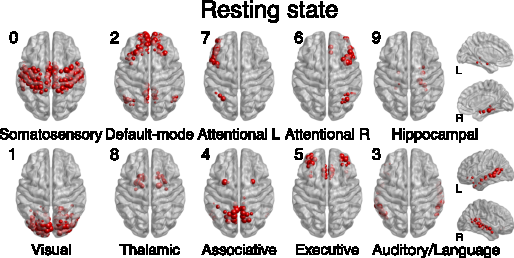
\includegraphics[width=1\linewidth]{images/figure_4_resting_state_communities.pdf}
\caption{The ten largest modules found by Surprise in the resting state network overlaid on an MRI brain template. The module indexes are ordered by decreasing size. The modules are named after corresponding functional networks previously identified by multivariate analysis of resting state fMRI data.}
\label{fig:figure_4_resting_state_communities}
\end{figure}

\begin{figure}[htb!]
\centering
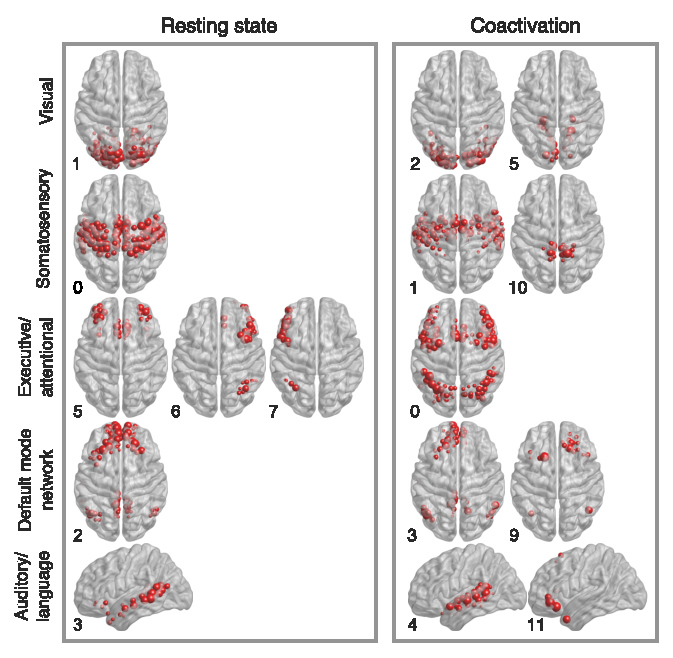
\includegraphics[width=1\linewidth]{images/figure_5_communities_comparison.pdf}
\caption{Comparison of selected modules in the partition obtained by Surprise in the resting state and coactivation networks. The indexes are inversely ranked according to the size of the modules in their respective networks.}
\label{fig:figure_5_communities_comparison}
\end{figure}

\begin{figure}[htb!]
\centering
\includegraphics[width=1\linewidth]{images/coact_rs_gamma_1_75.png}
\caption{Partitions obtained with multiresolution Modularity (Reichardt and Bornholdt method) for a value of the resolution parameter $\gamma=1.75$ for the coactivation and resting state networks. Increasing the resolution parameter improves detection of smaller modules, but breaks up larger ones, thus resulting in relatively homogeneous size distributions.}
\label{fig:figure_11_gamma_1_75_rs_coact}
\end{figure}

\begin{table}
\centering
\begin{tabular}{ccccc}
& & \textbf{Coactivation} & \\
\hline 
\textbf{NMI} &Modularity & Surprise & Infomap & RB $\gamma=1.75$ \\
\hline
Modularity 			& \textbf{1.00} & 0.61 & 0.56 & 0.61 \\
Surprise 			& 0.61 & \textbf{1.00} & 0.54 & 0.62 \\
Infomap 			& 0.56 & 0.54 & \textbf{1.00} & 0.59 \\
RB $\gamma=1.75$ 	& 0.59 & 0.61 & 0.59 & \textbf{1.00} \\ \hline 
\end{tabular}
\caption{Normalized Mutual Information between partitions of the coactivation network with Newman's Modularity, Infomap, Reichardt and Bornholdt and Surprise.
We used the Fagso algorithm for Surprise maximization, the \texttt{igraph} implementation of Infomap, the Brain Connectivity Toolbox implementation for RB (\texttt{community\_louvain.m} function) and \texttt{modularity\_und.m} for Modularity.
For each method the best solution over 100 repetitions was used to calculate NMI.}
\label{tab:coact_nmi_fagso}
\end{table}

\begin{table}
\centering
\begin{tabular}{ccccc}
& & \textbf{Resting State} & \\
\hline 
\textbf{NMI} &Modularity & Surprise & Infomap & RB $\gamma=1.75$ \\
\hline
Modularity & \textbf{1.00} & 0.52 &  0.70 & 0.66 \\
Surprise & 0.52 & \textbf{1.00} & 0.53 & 0.58 \\
Infomap & 0.70 & 0.53 & \textbf{1.00} & 0.68 \\
RB $\gamma=1.75$ & 0.66 & 0.58 & 0.68 & \textbf{1.00} \\ \hline 
\end{tabular}
\caption{Normalized Mutual Information between partitions of the Resting state network with Newman's Modularity, Infomap, Reichardt and Bornholdt and Surprise.
We used the Fagso algorithm for Surprise maximization, the \texttt{igraph} implementation of Infomap, the Brain Connectivity Toolbox implementation for RB (\texttt{community\_louvain.m} function) and \texttt{modularity\_und.m} for Modularity.
For each method the best solution over 100 repetitions was used to calculate NMI.}
\label{tab:rs_nmi_fagso}
\end{table}

% \begin{table}
% \centering
% \begin{tabular}{lccccc}
% & &\textbf{Coactivation}	&	&	&\\
% \hline
% &\textbf{NMI}&	Surprise &	Infomap&	RB $\gamma=1.75$\\ \hline
% \textbf{RS} &Surprise& 0.59&0.40&0.52\\
% 	&Infomap & 0.54&0.44&0.51\\
% 	&RB $\gamma=1.75$ &0.59&0.41&0.53\\ \hline 
% \end{tabular}
% \caption{Normalized Mutual Information between Resting State (RS) and Coactivation (Coact) partitions. Infomap and RB methods are repeated 100 times and partitions with the highest quality are used. NMIs are approximated to second significant digit.}
% \end{table}

The largest communities of the resting state network correspond to the primary sensorimotor cortex~\cite{biswal1995}, primary visual and extra-striate visual network, fronto-parietal lateralized networks~\cite{smith2009} as well as the so-called default mode network (DMN)~\cite{raichle2001,fransson2006}.
The attentional frontoparietal networks (FPAN)~\cite{beckmann2005} were detected as two separate, lateralized subnetworks, in agreement with~\cite{deluca2006} although other studies have identified a single, bilateral FPAN~\cite{markett2014}.

Smaller networks, like the executive control and auditory networks~\cite{salvador2005,vandenheuvel2010} were also resolved by Surprise, as well as subcortical structures, like the hippocampal and thalamic formations~\cite{roy2009,chen2013}. Interestingly, the thalamic nuclei appear as one tight community, despite the fact that they are structurally unconnected, in keeping with the idea that functional connectivity does not necessarily require the presence of strong structural links.

The more accurate partition afforded by Surprise may enable identification of differences in the modular structures of networks that cannot be appreciated with a resolution limited method. By way of example, I have compared the partitions of the resting state and coactivation networks (Figure \ref{fig:figure_5_communities_comparison}). Indeed, these networks are of a different nature, the former representing intrasubject baseline fluctuations in the brain's resting state, and the latter the responses to a variety of different tasks across subjects. However, Newman's Modularity finds similar partitions for these two networks, with 4 large modules each.

Conversely, under Surprise maximization, the partition of the resting state network shows many more small communities comprising less than 5 nodes (32 in total) compared with the coactivation one (only 11). Moreover, certain communities of the resting state network appeared to be split into smaller modules in the coactivation matrix. 
By way of example, the cuneus and the lingual and pericalcarine gyri were part of the occipital visual module in the resting state, but not in the coactivation network, where they formed a separate community (first row of Figure \ref{fig:figure_5_communities_comparison}).
Similarly, the precuneus and medial parts of the postcentral gyrus were identified as an independent community in the coactivation network, while they were part of the broad somatosensory network in the resting state connectivity graph~\cite{rubinov2011} (second row of Figure \ref{fig:figure_5_communities_comparison}).
Interestingly, the Broca area, indicated as Module 11 in Figure \ref{fig:figure_5_communities_comparison}, was separated from the auditory network in the coactivation network, and identified as a small, but anatomically and functionally distinct, community.
Conversely, other communities were split in the resting state but not in the coactivation network. The executive and attentional control networks were merged into a large community in the coactivation network, while they were separated under resting state conditions, including a subdivision of the left and right fronto-parietal networks (third row of Figure \ref{fig:figure_5_communities_comparison}).

While the resting state and coactivation networks appeared to possess virtually identical modular structures under Newman's analysis, they showed functionally and anatomically relevant differences when analyzed by Surprise maximization, with a Normalized Mutual Information between the partitions of the two networks of 0.5922. Indeed, Modularity tends to assign small communities to larger structures even when they correspond to tightly-knit modules, thus concealing differences in the graphs' modular structures that involve aggregation or disaggregation of smaller clusters. It is conceivable that the detrimental effects arising from the resolution limit may have affected previous studies comparing different populations~\cite{meunier2010}.
Surprise may offer a sharper tool to detect alterations of brain connectivity induced, for example, by psychiatric or neurological conditions, thus enabling the exploration of novel markers of brain disease.

%%%%%%%%%%%%%%%%%%%%%%%%%%%%%%%%%%%%%%%%%%%%%%%%%%%%%%%%%%%%%%%%%%%%%%%%%%%%%%
%%%%%%%%%%%%%%%%%%%%%%% HUBS CLASSIFICATION %%%%%%%%%%%%%%%%%%%%%%%%%%%%%%%%%%
%%%%%%%%%%%%%%%%%%%%%%%%%%%%%%%%%%%%%%%%%%%%%%%%%%%%%%%%%%%%%%%%%%%%%%%%%%%%%%
\subsection{Hubs classification}
Besides the exploration of functional and anatomical segregation, understanding the modular structure of brain networks is critical for the interpretation and classification of the roles played by the nodes within the network structure~\cite{sporns2007}. Highly connected nodes, or hub nodes, are particularly important for their topological centrality, and function as integrators. Hubs that primarily connect to nodes within the same module are dubbed ``provincial hubs'', and nodes that connect different modules are referred to as ``connector hubs''. The former are thought to be responsible for the formation and stability of the modules, while the latter ensure integration of the activity of the different modules. Obviously, interpretation of the hub's role relies on the correct identification of the optimal network partition, and may be strongly affected by the resolution limit.

Here, I have performed a hub's role analysis for the resting state and coactivation networks under Modularity and Surprise maximization.
To this end, I have adopted Guimera' and Amaral classification scheme~\cite{guimera2005}, whereby nodes are classified by their within-community degree $z$ (a measure of how well-connected a node is to other nodes in the same community) and their participation coefficient $P$, a parameter that is $0$ for nodes with purely intra-module connections and $1$ for nodes whose links project primarily to other modules. 

Figures \ref{fig:figure_6_ga_rs_coact}A and \ref{fig:figure_6_ga_rs_coact}B show the different positioning of high-degree nodes in the Guimera' and Amaral plot for the coactivation and resting state networks partitioned using Newman’s approach and Surprise maximization. In this scheme, provincial hubs are high-degree nodes that score high $z$ and low $P$ values (\emph{R5} region); conversely, connector hubs are characterized by larger $P$ values (regions on the right-hand side of the plot).

\begin{figure}[ht!]
\centering
\includegraphics[width=0.5\linewidth]{images/figure_6_ga_rs_coact.pdf}
\caption{Classification of representative nodes according to their intra- and intermodule connections for the resting state (A) and coactivation (B) networks. Empty circles and full circles indicate the position of each node in the Guimera' and Amaral’s plot after partition by Modularity or Surprise, respectively. An overall increase in the participation coefficient, a measure of the intermodule connectivity, is observed for the Surprise partition relative to the Modularity partition. To avoid cluttering of the graph, I only reported those nodes with a degree higher than the average within a Standard Deviation, and whose classification is different in the two partitions. The abbreviations of the brain regions corresponding to the nodes are reported in the appendix, Table~\ref{tab:abbreviations}.}
\label{fig:figure_6_ga_rs_coact}
\end{figure}

A finer partition in smaller communities may be expected to determine an overall increase in participation coefficient and decrease in within-community degree. However, the heterogeneous partitions obtained by Surprise maximization resulted in non-trivial changes in the Guimera' and Amaral classification. By way of example, I discuss in greater detail two regions whose roles are very different in the two partitions, to highlight the effects of the resolution limit.

Nodes that belong in the hippocampal formation show a large within-module coefficient, and appear as provincial hubs (region R5 of Figure \ref{fig:figure_6_ga_rs_coact}) under Modularity optimization. However, their participation coefficient increases 6-fold in the partition by Surprise, which reveals a role as connectors for these nodes, with widespread projections to many other modules across the brain, including the module 3, 6, 8, 5, 2, corresponding to the DMN, the amygdala and parahippocampal formation, the temporal inferior gyrus, the cuneus and lingual gyrus, and the visual cortex, respectively.
This finding is in agreement with the idea that the hippocampus acts as ``network convergence zone'', as it receives polysensory input from distributed association areas in the neocortex~\cite{misic2014}.

Interestingly, the right shift in the Guimera-Amaral plot is less pronounced for the nodes in the posterior part of the hippocampus (Figure \ref{fig:figure_7_ga_coact_hippocampus}). A differential classification of the anterior and posterior hippocampus is consistent with the hypothesis of a functional differentiation of this structure~\cite{moser1998}, with the posterior hippocampus mostly involved in memory and cognition, and the anterior hippocampus playing a role in the processing of stress, emotion and affect~\cite{fanselow2010}. Moreover, studies in animal models have shown differential organization of the efferent connections of the hippocampal formation~\cite{swanson1977}, consistent with different functions for the anterior and posterior hippocampus.

\begin{figure}[htb!]
\centering
\includegraphics[width=0.5\linewidth]{images/figure_7_hippocampus.pdf}
\caption{Top panel: classification of all the hippocampal nodes according to the Guimera' and Amaral's scheme for the coactivation network. Empty circles and full circles indicate the position of each node after partition by Modularity or Surprise, respectively. Bottom panel: anatomical positions of the nodes in the hippocampal formation, colored by Surprise community membership. The increase in participation coefficient upon partition by Surprise is more pronounced for nodes in the anterior part of hippocampus, with an antero-posterior gradient.}
\label{fig:figure_7_ga_coact_hippocampus}
\end{figure}

Similar rightward shifts for nodes and hubs were observed in the resting state network, and reported in Figure \ref{fig:figure_6_ga_rs_coact}.
However, increases in participation coefficients are by no means the only differences in the classification of nodes obtained by Surprise maximization. A prominent example is the precuneus (PC) (Figure \ref{fig:figure_6_ga_rs_coact}B, blue dots) that shows a high participation coefficient in both partitions by Modularity and Surprise, but a much higher within-module degree under Surprise maximization.

Indeed, the nodes comprised in the precuneus intrinsically possess high inter-cluster connectivity, but are distributed among the four modules found by Modularity. In the partition by Surprise they are grouped together, and this precuneal module as a whole plays a connector's role integrating different communities (Figure \ref{fig:figure_8_ga_rs_precuneus}), a hypothesis that is consistent with the precuneus supporting a wide spectrum of highly integrated tasks, from visuo-spatial imagery to episodic memory retrieval and self-processing operations~\cite{cavanna2006}.

In summary, partition by Surprise maximization results in very different distributions of participation coefficients and within-module degree compared to Modularity. These differences are not uniform across nodes, and arise from the limited ability of Modularity to identify small modules. Finer partition by Surprise reveals very different roles for some key brain areas, and suggests that a systematic reanalysis of the topological roles of brain nodes and hubs may be in order.

\begin{figure}[htb!]
\centering
\includegraphics[width=0.5\linewidth]{images/figure_8_precuneus.pdf}
\caption{Top panel: classification of the precuneal nodes according to the Guimera' and Amaral's scheme for the resting state network. Empty circles and full circles indicate the position of each node after partition by Modularity or Surprise, respectively. Bottom panel: anatomical positions of the nodes in the precuneus, colored by Surprise community membership. The nodes in the dorsal part of the precuneus exhibit a sharp increase in within-module degree.}
\label{fig:figure_8_ga_rs_precuneus}
\end{figure}


%%%%%%%%%%%%%%%%%%%%%%%%%%%%%%%%%%%%%%%%%%%%%%%%%%%%%%%%%%%%%%%%%%%%%%%%
%%%%%%%%%%%%%% LIMITATIONS OF BINARY SURPRISE %%%%%%%%%%%%%%%%%%%%%%%%%%
%%%%%%%%%%%%%%%%%%%%%%%%%%%%%%%%%%%%%%%%%%%%%%%%%%%%%%%%%%%%%%%%%%%%%%%%
\section{Limitations of binary Surprise}
A potential limitation of Surprise is related to its definition in terms of discrete probability distributions. This makes Surprise suited for the study of binarized networks. While the topological backbones of the networks I have investigated appear quite robust against removal of lowest-weight edges and binarization, as shown by our percolation and stability analyses (Figures~\ref{fig:figure_8_percolation_analysis},~\ref{fig:figure_9_rs_threshold_study},~\ref{fig:figure_10_rs_threshold_study}), the application of its weighted counterpart, Asymptotical Surprise, will help overcome the need of binarization.

The superior resolution afforded by Surprise may make it more vulnerable than other methods to noise and experimental errors. Indeed, occasional misassignment of nodes due to noise-induced changes in edge distribution are likely to affect small modules, comprising only a few nodes, more than large ones. Hence, experimental uncertainty also limits resolution, and a resolution-limit-free method would not necessarily improve the quality of the partition in a scenario dominated by noise. 

To ascertain whether this is the case for the co-activation and resting state networks investigated here, I have simulated the effects of experimental errors by injecting noise into the distributions of weights prior to the binarization procedure, thus introducing variability in the connectivity structure of the resulting binary networks.
We set levels of noise sufficient to perturb up to 10\% of the edges of the final binary network. Using this procedure, for each level of noise I generated ten different graphs, and applied the Surprise Maximization algorithm to each of them. 

The ten different graphs were generated by adding noise to the off-diagonal elements of the adjacency matrix prior to the binarization procedure. The amplitude of noise was chosen to randomly perturb 10\% of the edges after binarization. Surprise maximization was applied to the resulting graphs. In the left panel of Figure~\ref{fig:figure_9_nmi}, I reported the Normalized Mutual Information (NMI) between the optimal partitions of each of the ten perturbed networks and that of the original resting state network.
The number of communities retrieved by FAGSO in each of the perturbed networks is reported in the right panel of Figure~\ref{fig:figure_9_nmi}. The graphs show that the partitions of the ``noisy'' graphs are consistent and similar to those of the unperturbed network, with NMI scores close to 1 and almost constant numbers of communities.
These results demonstrate that Surprise maximization can retrieve the network's community structure even in the presence of substantial noise in the data.
We found that the partitions of these graphs were highly consistent with those of the original networks (Figure~\ref{fig:figure_9_nmi}).

\begin{figure}[ht]
\centering
\includegraphics[width=1\linewidth]{images/figure_9_nmi.png}
\caption{Assessment of the effects of experimental error on the community structure of the resting state network.}
\label{fig:figure_9_nmi}
\end{figure}

We should also stress that there is no constraint in the FAGSO algorithm imposing inter-hemispherical symmetry of the partition.
Nevertheless, I observed homotopic correspondence in the community structure, and a close resemblance with established neurofunctional circuits as in Figure~\ref{fig:figure_4_resting_state_communities} and~\ref{fig:figure_5_communities_comparison}. Taken together, simulations of the effects of noise and qualitative considerations on the neurofunctional significance of the modules identified by Surprise corroborate the idea that experimental error is not the predominant factor in the networks investigated.

A final and important point I should highlight is that Surprise maximization, in the implementation I have used here, does not allow for overlapping communities. Other methods have been applied to investigate this aspect in brain networks~\cite{palla2005,ahn2010}. However, a recent comparative analysis of graph partitioning algorithms on a variety of benchmark networks~\cite{lancichinetti2009} has shown that these methods are also prone to merging overlapping communities, with relatively modest performance in recovering heterogeneous cluster distributions planted in model networks.
Despite these potential limitations, the resolution-limit-free behavior of Surprise makes it an excellent tool to explore and to overcome the effects of the resolution limit in the modular structure of brain connectivity networks.


%%%%%%%%%%%%%%%%%%%%%%%%%%%%%%%%%%%%%%%%%%%%%
%%%%%%%%%%%%%% CONCLUSIONS %%%%%%%%%%%%%%%%%%
%%%%%%%%%%%%%%%%%%%%%%%%%%%%%%%%%%%%%%%%%%%%%
\section{Conclusions}
In conclusion, I have shown that Surprise, a recently proposed fitness function for graph partitioning, behaves like a resolution-limit-free function.
I have applied Surprise maximization to study the modular structures of two different brain networks.
Surprise maximization resulted in partitions comprising communities of widely distributed sizes, consistent with the idea that small and large modules coexist in brain networks.
Moreover, the finer partition afforded by Surprise made it possible to appreciate differences in the modular structures of diverse brain networks that were undetected by resolution limited methods like Newman's Modularity.
Finally, the use of Surprise revealed the deleterious effects of the resolution limit in the classification of nodal roles.
Altogether, these results indicate that the resolution limit may have substantially affected many of the analyses of brain connectivity networks reported in the literature, and call for a revisitation of some of the conclusions and models that have relied on Modularity maximization or similarly resolution-limited algorithms.
Surprise appears as a promising alternative method that appeals to the intuition that tightly-knit clusters of nodes represent legitimate structural
or functional modules independently of their size.